\section{Math 202A - HW13 - Dan Davison - \texttt{ddavison@berkeley.edu}}

\begin{mdframed}
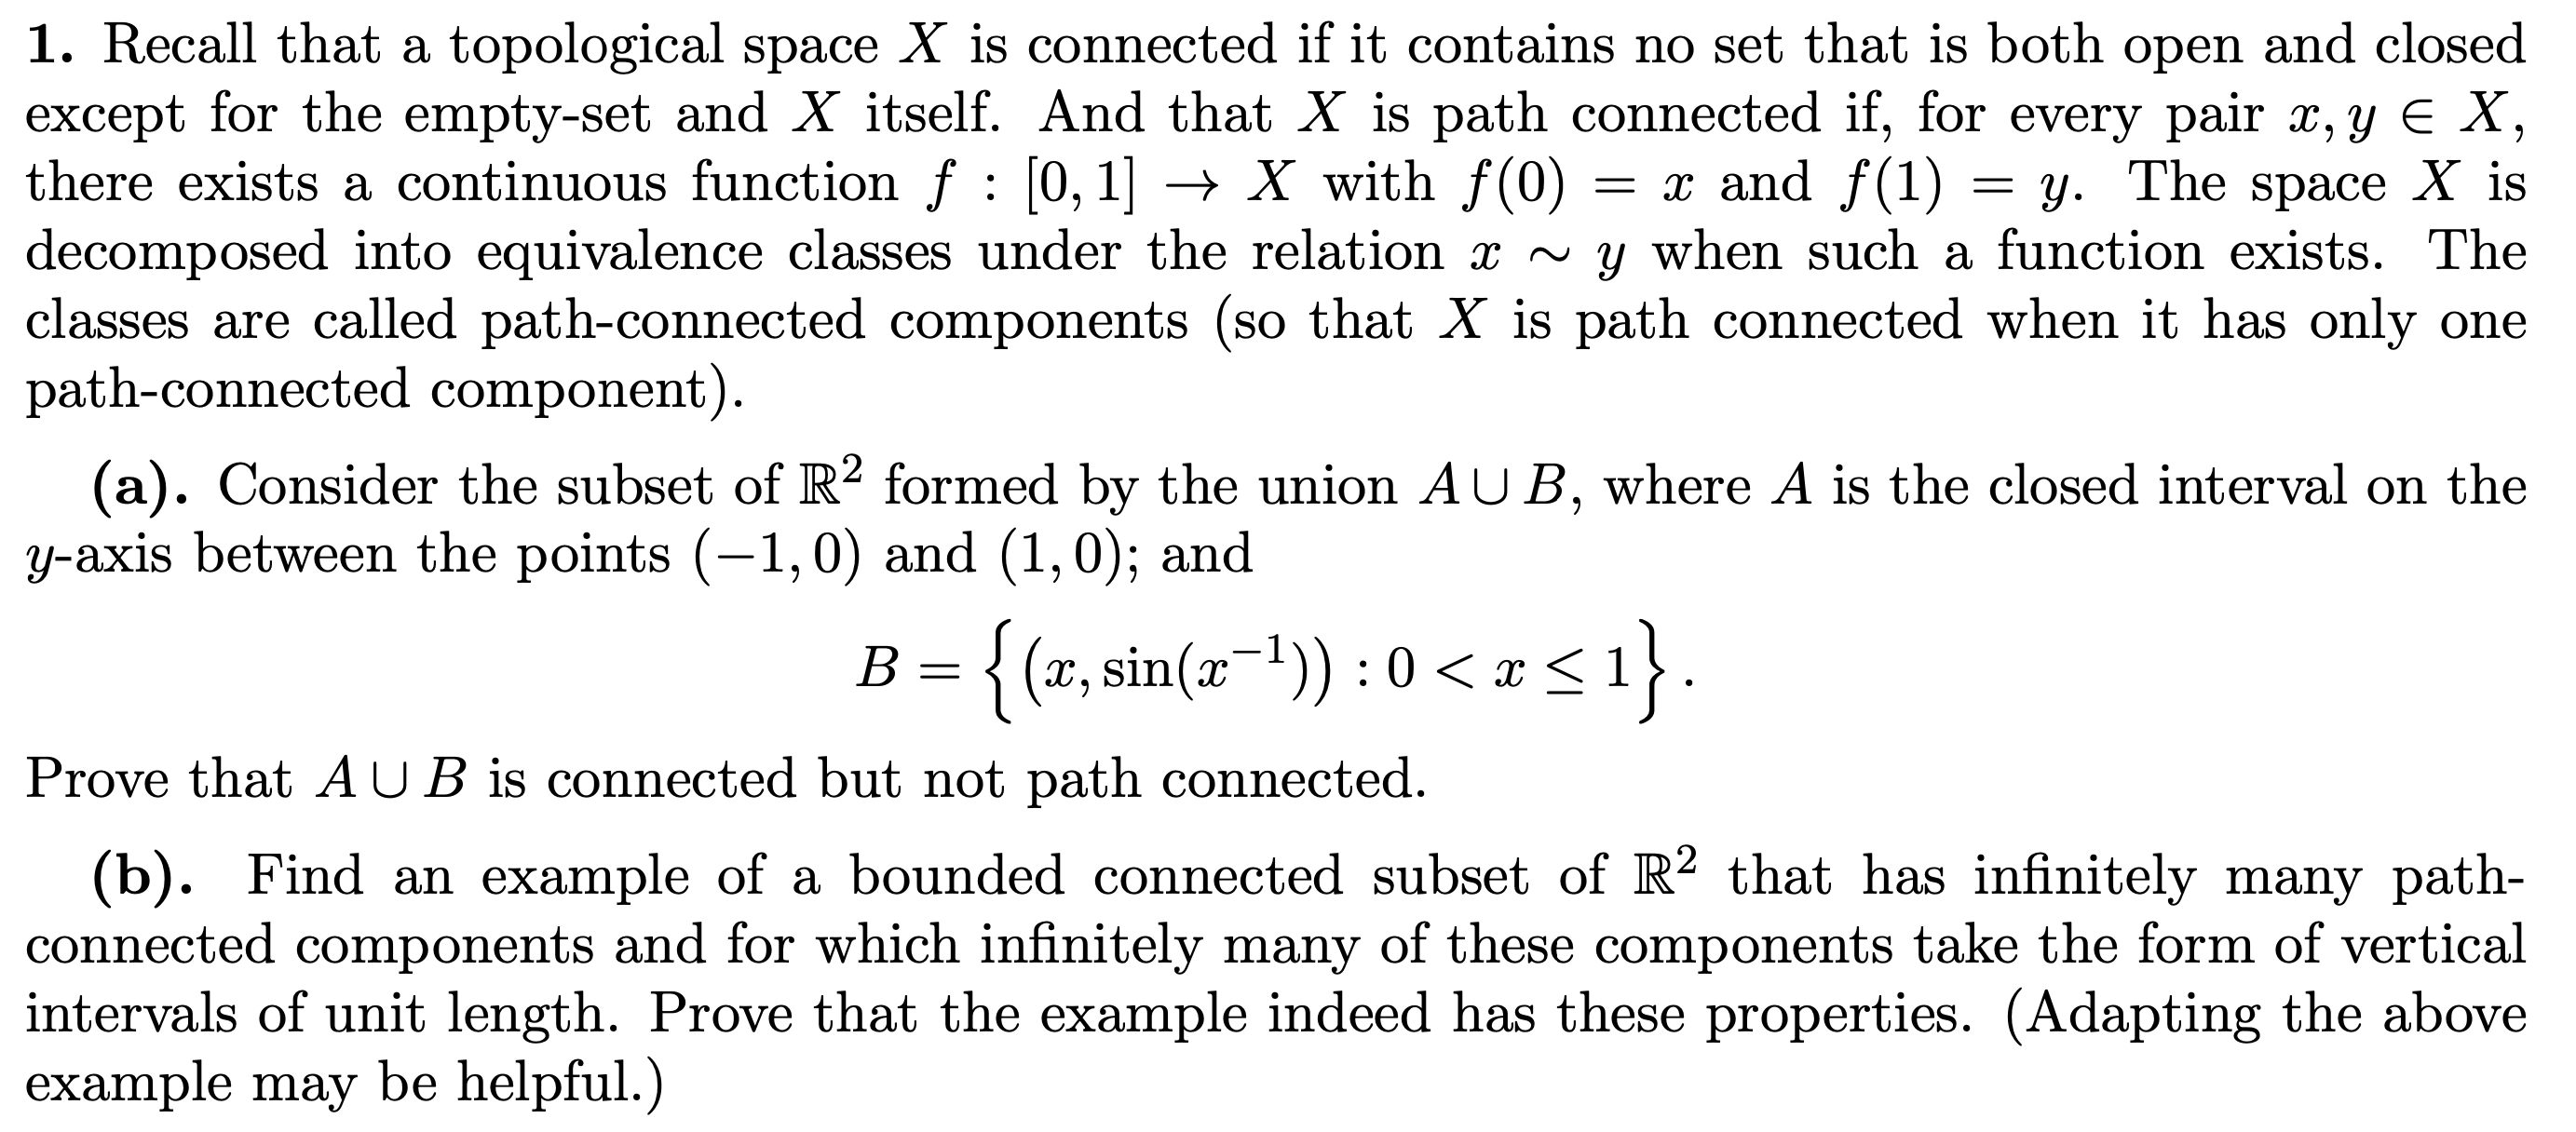
\includegraphics[width=400pt]{img/analysis--berkeley-202a-hw13-26dd.png}
\end{mdframed}

\begin{enumerate}[label=(\alph*)]
\item
  \begin{claim*}
    $A \union B$ is connected.
  \end{claim*}

  \begin{proof}
    We must show that $A \union B$ cannot be written as the union of two disjoint non-empty open sets.

    Suppose for a contradiction that $U$ and $V$ are disjoint open sets such that $U \union V = A \cup B$.
    Let $z \in B$ and without loss of generality suppose that $z \in V$. Then $B \subseteq V$ (since $B$ is
    connected). Note that the open ball at $(0, 0)$ contains a point of $B$. But $U$ and $V$ are disjoint,
    therefore $(0, 0) \in V$. But $(0, 0) \in A$ and $A$ is connected, so $A \subseteq V$.
    Therefore $A \union B = V$. But this is a contradiction since $U$ and $V$ are disjoint and non-empty.
    Therefore $A \union B$ are connected.
  \end{proof}


  \begin{claim*}
    $A \union B$ is not path-connected.
  \end{claim*}

  \begin{proof}
    Suppose for a contradiction that there exists a continuous function $f: [0, 1] \to A \union B$ such
    that $f(0) = (0, 1)$ and $f(1) = (0, 0)$.

    Write $f = (f_x, f_y)$ where $f_x: [0, 1] \to [0, 1]$ and $f_y: [0, 1] \to [-1, 1]$ give the coordinates of $f$.

    Let $\eps > 0$ and let $(t_n)_{n=1}^\infty$ be an increasing sequence with $0 < t_n < 1$ and $t_n \to 1$.
    Then $f_y(t_n) \to 0$ since $f$ is continuous. Let $N$ be such that $f_y(t_n) < \eps$ for all $n \geq N$. But
    this is a contradiction since $f_y (t_n))$ is oscillating between $-1$ and $1$ but $\eps$ is arbitrary.
    Therefore no such continuous function $f$ exists.

    \red{TODO} make this rigorous.
  \end{proof}
\item

  Informally, we will take vertical intervals positioned at each point of a countably infinite sequence of
  rationals and between each successive pair, place a variant of the ``topologist's sine curve​'' constructed so
  that it ``speeds up​'' in both directions. The resulting topological space will be connected but not
  path-connected, because we have seen above that that is what happens when the topologist's sine curve
  approaches a vertical interval.

  Let $\N$ be the natural numers excluding $0$.

  Let $q_n = \sum_{i=1}^n 2^{-n} \in \Q \cap [\frac{1}{2}, 1)$. Then $\{q_n ~:~ n \in \N\}$ is a countably
  infinite set of rationals in $[\frac{1}{2}, 1)$.

  Let $I_n = \{q_n\} \times [0, 1] \subset U$. This is a vertical interval of unit length.

  Let $m_n = (q_{n+1} - q_n)/2$ and let $S_n = \{\sin\((|x - m_n| - m_n)^{-1}\) ~:~ x \in (q_n, q_{n+1})\}$. We
  will refer to this as a ``bidirectional topologist's sine curve​''.

  Finally, let $U = \{I_n ~:~ n \in \N\} \union \{S_n ~:~ n \in \N\}$.

  Informally, $U$ consists of a countable collection of vertical intervals together with a ``bidirectional
  topologist's sine curve​'' between each successive pair of vertical intervals.


  \begin{claim}
    $U$ is a bounded and connected subset of $\R^2$.
  \end{claim}

  \begin{proof}
    $U \subset [0, 1]^2 \subset \R^2$ therefore $U$ is a bounded subset of $\R^2$.

    Recall that we proved above that $V := \(\{0\} \times [0, 1]\) \union \{\sin(1/x) ~:~ x \in (0, 1]\}$ is a
    connected topological space.

    It follows that $I_n \union S_n$ is connected for all $n$ (formally, I believe we can prove this by
    exhibiting a homeomorphism between $V$ and $I_n \union S_n$ and noting that a topological space is
    connected if it is homeomorphic to a different connected topological space. Or possibly I would have to use
    just the ``first half​'' of $S_n$, i.e. $I_n \cup \(S_n \cap \((q_n, m_n) \times [0, 1]\)\)$)

    Similarly, it follows that $S_n \cup I_{n+1}$ is connected for all $n$ (the geometry is identical but with
    left-right orientation reversed).

    It then follows by induction that $U$ is connected.
  \end{proof}

  \begin{claim}
    $U$ has infinitely many path-connected components and infinitely many of these take the form of a vertical
    interval of unit length.
  \end{claim}

  \begin{proof}
    Let $I_n = \{q_n\} \times [0, 1] \subset U$. This is a vertical interval of unit length. Clearly, $I_n$ is
    path-connected. To see this, let $(q_n, y_1), (q_n, y_2) \in I_n$ and without loss of generality suppose
    that $y_1 < y_2$. - Then $f: [0, 1] \to I_n$ defined by $f(t) = (q_n, y_1 + t(y_2 - y_1))$ has the property
    that $f(0) = (q_n, y_1)$ and $f(1) = (q_n, y_2)$.

    Recall that $S_n$ is a ``bidirectional topologist's sine curve​'' in the current construction, and recall also
    that we proved above that $\(\{0\} \times [0, 1]\) \union \{\sin(1/x) ~:~ x \in (0, 1]\}$ is not path
    connected. It follows that neither $I_n \union S_n$ nor $I_n \union S_{n-1}$ is path-connected, and it
    follows from this that $I_n \union I_{m}$ is not path-connected for all $n \neq m$. We
    have $\bigcup_{n \in \N} I_n \subset U$, therefore $U$ contains infinitely many path-connected components
    which take the form of a vertical interval of unit length.
  \end{proof}
\end{enumerate}



\newpage
\begin{mdframed}
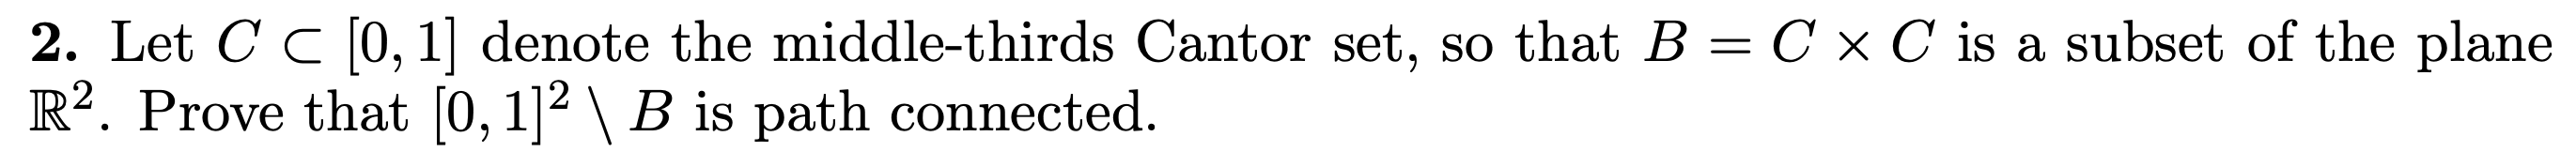
\includegraphics[width=400pt]{img/analysis--berkeley-202a-hw13-e2f7.png}
\end{mdframed}

Note: the notation $(a, b)$ refers to a point in $[0, 1]^2$ throughout; never an open interval.

Let $A \subset [0, 1]$ be a strict subset of $[0, 1]$.

\begin{definition*}
  We define, in the context of this problem, a {\em path} between points $(x_1, y_1)$ and $(x_2, y_2)$ to be a
  continuous function $f:[0, 1] \to \([0, 1]^2 \setminus (A \times A)\)$ such that that $f(0) = (x_1, y_1)$
  and $f(1) = (x_2, y_2)$.

  Suppose $f$ is a path ending at $a$ and $g$ is a path starting at $a$. Then we define the {\em concatenation}
  of paths $f$ and $g$ to be the function $f \oplus g$ defined by
  \begin{align*}
    (f \oplus g)(t) =
    \begin{cases}
      f(2t)           &t < 0.5 \\
      g(2t - 1)   &t \geq 0.5.
    \end{cases}
  \end{align*}
  We define a {\em crossroad point} to be a point $(x, y)$ such that $x \in [0, 1] \setminus A$
  and $y \in [0, 1] \setminus A$.
\end{definition*}

We now prove the main claim; the necessary lemmas are proved below.

\begin{proof}
  Let $(x_1, y_1)$ and $(x_2, y_2)$ be two arbitrary points of $[0, 1]^2 \setminus (A \times A)$.

  Let $u$ and $v$ be crossroad points. Then there exists a path $f$ from $(x_1, y_1)$ to $u$, a path $g$
  from $u$ to $v$, and a path $h$ from $v$ to $(x_2, y_2)$, by lemmas \ref{point-to-crossroad},
  \ref{crossroad-to-crossroad}, and \ref{symmetry}.

  Therefore $(f \oplus g) \oplus h$ is a path between $(x_1, y_1)$ and $(x_2, y_2)$.

  Therefore $[0, 1]^2 \setminus (A \times A)$ is path-connected for any strict subset $A \subset [0, 1]$.
  Therefore it is true for the particular choice of $A = C$, the middle-thirds Cantor set.
\end{proof}


\begin{lemma}\label{concatenation}
  The concatenation of two paths is a path.
\end{lemma}

\begin{proof}
  Let $f$ be a path from $a$ to $b$ and let $g$ be a path from $b$ to $c$. Then we
  have $(f \oplus g)(0) = f(0) = a$ and $(f \oplus g)(1) = g(1) = c$.

  We must show continuity. We have that $f \oplus g$ is continuous at all
  points $t \in [0, 1] \setminus \{0.5\}$, since $f$ and $g$ are continuous (therefore for a given $t$,
  any $\delta < |t - 0.5|$ will do.) Let $t = 0.5$. Then $f \oplus g$ is continuous at $t$ from the left due to
  the continuity of $f$ and continuous at $t$ from the right due to the continuity of $g$. Let $\delta_L$ be
  the $\delta$ that works to the left and $\delta_R$ be the $\delta$ that works to the right.
  Then $\min(\delta_L, \delta_R)$ works at $t$.

  Therefore $f \oplus g$ is a path from $a$ to $c$.
\end{proof}

\begin{lemma}\label{symmetry}
  If there exists a path from $a$ to $b$ then there exists a path from $b$ to $a$.
\end{lemma}

\begin{proof}
  Let $f$ be a path from $a$ to $b$. Then $g(t) = f(1 - t)$ satisfies $g(0) = b$ and $g(1) = a$ and is
  continuous since $f$ is continuous.
\end{proof}

\begin{lemma}\label{crossroad-to-same-row-column}
  Let $(x_1, y_1)$ be a crossroad point. Then a path exists connecting $(x_1, y_1)$ to $(x_1, y)$ for
  every $y \in [0, 1]$. Similarly, a path exists connecting $(x_1, y_1)$ to $(x, y_1)$ for
  every $x \in [0, 1]$.
\end{lemma}

\begin{proof}
  Let $y \in [0, 1]$. Then $f:[0, 1] \to \([0, 1]^2 \setminus (A \times A)\)$ defined by
  \begin{align*}
    f(t) = \(x_1, (y_1 + t(y - y_1))\)
  \end{align*}
  is clearly continuous and thus a path connecting $(x_1, y_1)$ to $(x_1, y)$.

  Similarly, let $x \in [0, 1]$. Then
  \begin{align*}
    f(t) = \(x_1 + t(x - x_1), y_1\)
  \end{align*}
  is a path connecting $(x_1, y_1)$ to $(x, y_1)$.
\end{proof}

\begin{lemma}\label{crossroad-to-crossroad}
  A path exists connecting any two crossroad points $(x_1, y_1)$ and $(x_2, y_2)$.
\end{lemma}

\begin{proof}
  By lemma \ref{crossroad-to-same-row-column} a path $f$ exists from $(x_1, y_1)$ to $(x_1, y_2)$ and a
  path $g$ exists from $(x_2, y_2)$ to $(x_1, y_2)$. Then $f \oplus g$ is a path connecting the two crossroad
  points.
\end{proof}

\begin{lemma}\label{point-to-crossroad}
  Let $(x, y) \in \([0, 1]^2 \setminus (A \times A)\)$. Then there exists a path from $(x, y)$ to a
  crossroad point.
\end{lemma}

\begin{proof}
  We have that $x \in [0, 1] \setminus A$ or $y \in [0, 1] \setminus A$. Suppose without loss of generality
  that $x \in [0, 1] \setminus A$. Pick a point $y' \in [0, 1] \setminus A$. Then $(x, y')$ is a crossroad
  point and there exists a path from $(x, y)$ to $(x, y')$ by lemma \ref{crossroad-to-same-row-column}
\end{proof}


\newpage
\begin{mdframed}
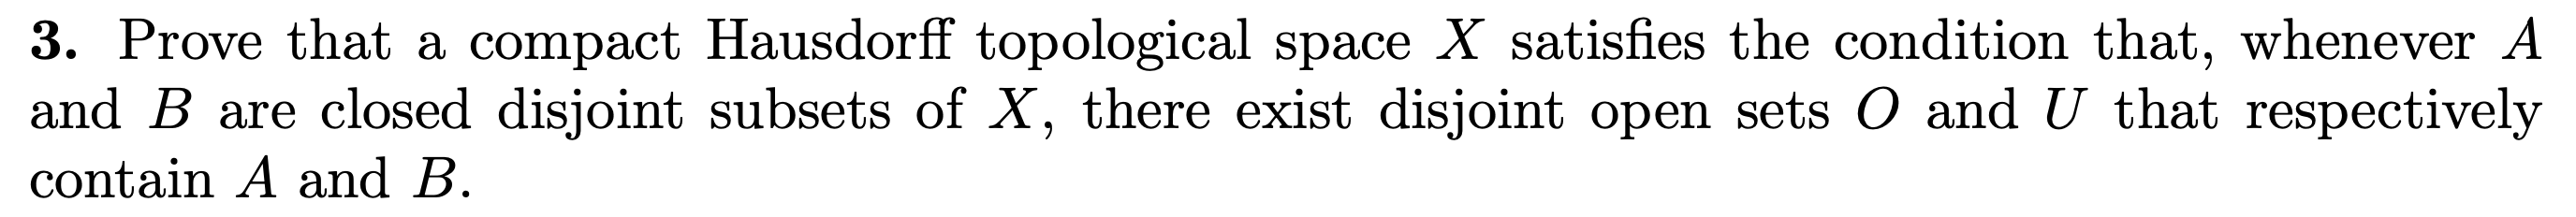
\includegraphics[width=400pt]{img/analysis--berkeley-202a-hw13-983a.png}
\end{mdframed}

\begin{proof}
  This is theorem 20.30 of Bass; the proof is given there. The theorem states that if $X$ is compact Hausdorff
  then $X$ is normal, and the conditions asked for here are satisfied by the definition of normal.\\
  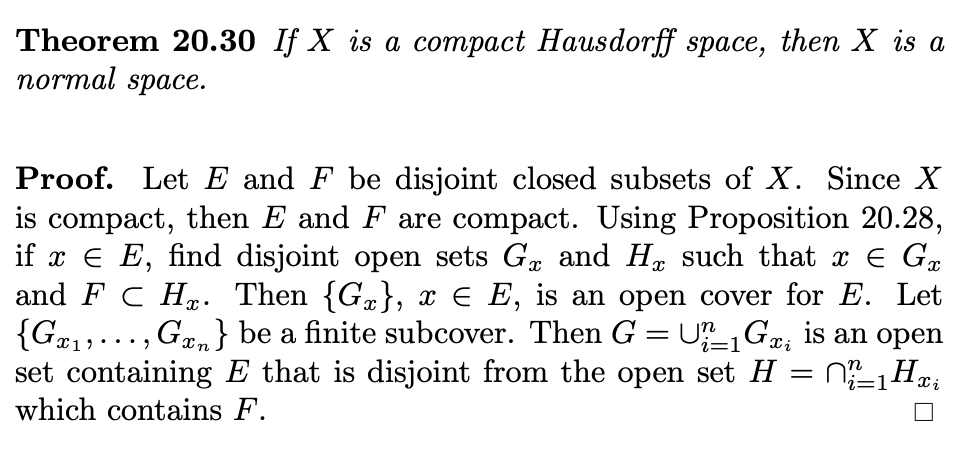
\includegraphics[width=400pt]{img/analysis--berkeley-202a-hw13-7531.png}
\end{proof}


\newpage
\begin{mdframed}
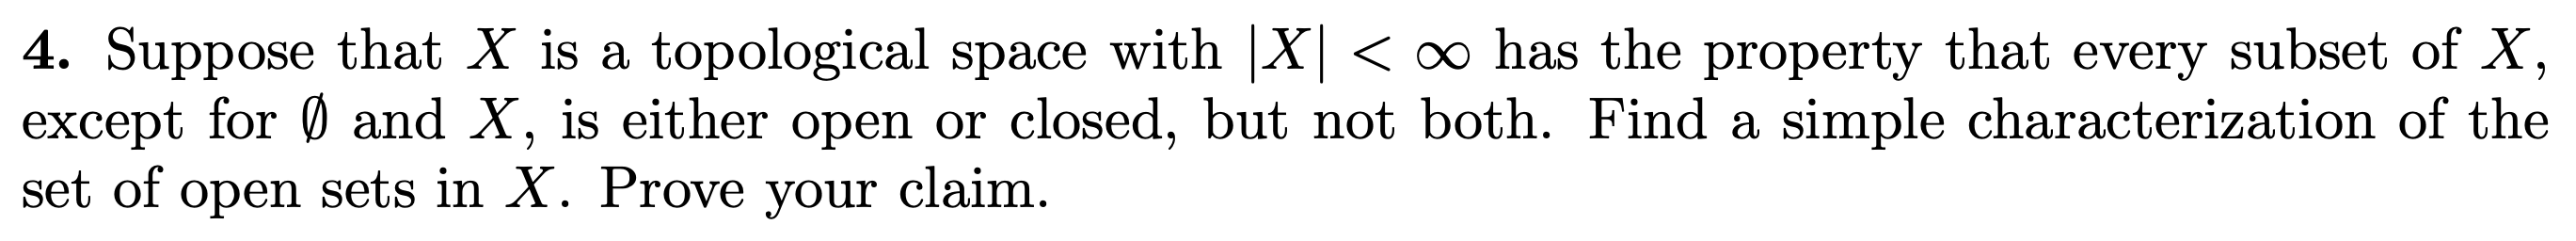
\includegraphics[width=400pt]{img/analysis--berkeley-202a-hw13-9356.png}
\end{mdframed}

% From Aidan Backus (grader):

% Recall that a directed graph is "transitive" if given edges x→y→z we can compose them to get an
% edge x→z. The key point is that if X is a finite topological space then we can think of X as (the
% vertices of) a transitive directed graph. Namely, if x,y∈X then we define an edge x→y iff x is in
% the closure of y. Conversely, if X is a transitive directed graph we can put a topology on (the
% vertices of) X by saying that the open sets are the sets which are closed upwards.

% The following are equivalent: X is connected (in the sense of topological spaces); and X is
% graph-theoretically connected. Indeed, every graph-theoretically connected component of X is a
% closed subset of X, so it is clopen since its complement is closed; the converse is similar.

% If X is as in the problem and there is an edge x→y then either x=y or there is no edge y→x. Suppose
% that there are edges x→y→x. Then x, y have the same closure, so x, y are indiscernible. Therefore
% {x} is not open, so it is closed, so it is the closure of x, so x=y.

% Suppose that every proper nonempty subset of X is either open or closed but not open. Then X has no
% proper nonempty clopen subsets, so X is connected, and hence graph-theoretically connected. By the
% previous paragraph, X has no cycles except for the trivial edges x→x. I think that one can now show
% that there is a unique vertex x such that either x is initial or x is final. To do this, you first
% might show that X is the transitive closure of a directed tree.

% If x is initial, then x is in the closure of every point. So every set that contains x is open and
% every other set is closed. Otherwise, x is final; by symmetry (since we're in a finite topological
% space, the set of closed sets is also a topology!) every set that contains x is closed and every
% other set is open.


First, let's examine some small finite sets and the possible topologies that meet the specified
condition. The following table excludes topologies that differ only by a relabeling of the elements
in the underlying set.

[Incomplete, table is incomplete and I didn't figure out what the pattern was.]

\begin{tabular}{l|l|l}
  set&non-trivial&non-trivial\\
     &open subsets&closed subsets \\
  \hline
  $\{\}$             &                                                                                                 & \\
  \hline
  $\{1\}$            &                                                                                                 & \\
  \hline
  $\{1, 2\}$         & $\{1\}$                                                                                         & $\{2\}$\\
  \hline
  $\{1, 2, 3\}$      & $\{1\}$                                                                                         & $\{2, 3\}$ \\
  $\{1, 2, 3\}$      & $\{1\}, \{2\}, \{1, 2\}$                                                                        & $\{2, 3\}, \{1, 3\}, \{3\}$ \\
  $\{1, 2, 3\}$      & $\{1\}, \{1, 2\}$                                                                               & $\{2, 3\}, \{3\}$ \\
  $\{1, 2, 3\}$      & \sout{$\{1\}, \{2, 3\}$}                                                                        & \sout{$\{2, 3\}, \{1\}$} \\
  $\{1, 2, 3\}$      & $\{1, 2\}$                                                                                      & $\{3\}$ \\
  $\{1, 2, 3\}$      & \sout{$\{1\}, \{2\}, \{1, 2\}, \{3\}, \{1, 3\}, \{2, 3\}$}                                      & \sout{$\{2, 3\}, \{1, 3\}, \{3\}, \{1, 2\}, \{2\}, \{1\}$} \\
  $\{1, 2, 3\}$      & \sout{$\{1\}, \{2\}, \{1, 2\}, \{1, 3\}$}                                                       & \sout{$\{2, 3\}, \{1, 3\}, \{3\}, \{2\}$} \\
  \hline
  $\{1, 2, 3, 4\}$   & $\{1\}$                                                                                         & $\{2, 3, 4\}$ \\
  $\{1, 2, 3, 4\}$   & $\{1\}, \{2\}, \{1, 2\}$                                                                        & $\{2, 3, 4\}, \{1, 3, 4\}, \{3, 4\}$ \\
  $\{1, 2, 3, 4\}$   & $\{1\}, \{1, 2\}$                                                                               & $\{2, 3, 4\}, \{3, 4\}$ \\
  $\{1, 2, 3, 4\}$   & $\{1\}, \{2, 3\}, \{1, 2, 3\}$                                                                  & $\{2, 3, 4\}, \{1, 4\}, \{4\}$ \\
  $\{1, 2, 3, 4\}$   & $\{1\}, \{1, 2, 3\}$                                                                            & $\{2, 3, 4\}, \{4\}$ \\
  $\{1, 2, 3, 4\}$   & \sout{$\{1\}, \{2, 3, 4\}$}                                                                     & \sout{$\{2, 3, 4\}, \{1\}$} \\
  $\{1, 2, 3, 4\}$   & $\{1, 2\}$                                                                                      & $\{3, 4\}$ \\
  $\{1, 2, 3, 4\}$   & \sout{$\{1, 2\}, \{3, 4\}$}                                                                     & \sout{$\{3, 4\}, \{1, 2\}$} \\
  $\{1, 2, 3, 4\}$   & $\{1\}, \{2\}, \{1, 2\}, \{3\}, \{1, 3\}, \{2, 3\}, \{1, 2, 3\}$                                & $\{2, 3, 4\}, \{1, 3, 4\}, \{3, 4\}, \{1, 2, 4\}, \{2, 4\}, \{1, 4\}, \{4\}$ \\
  $\{1, 2, 3, 4\}$   & \sout{$\{1\}, \{2\}, \{1, 2\}, \{3\}, \{1, 3\}, \{2, 3\}, \{1, 2, 3\}$},                        & \sout{$\{2, 3, 4\}, \{1, 3, 4\}, \{3, 4\}, \{1, 2, 4\}, \{2, 4\}, \{1, 4\}, \{4\}$}, \\
                     & ~~~~\sout{$\{4\}, \{1, 4\}, \{2, 4\}, \{1, 2, 4\}, \{3, 4\}, \{1, 3, 4\}, \{2, 3, 4\}$}         & ~~~~\sout{$\{1, 2, 3\}, \{2, 3\}, \{1, 3\}, \{3\}, \{1, 2\}, \{2\}, \{1\}$} \\
\end{tabular}

\newpage
\begin{mdframed}
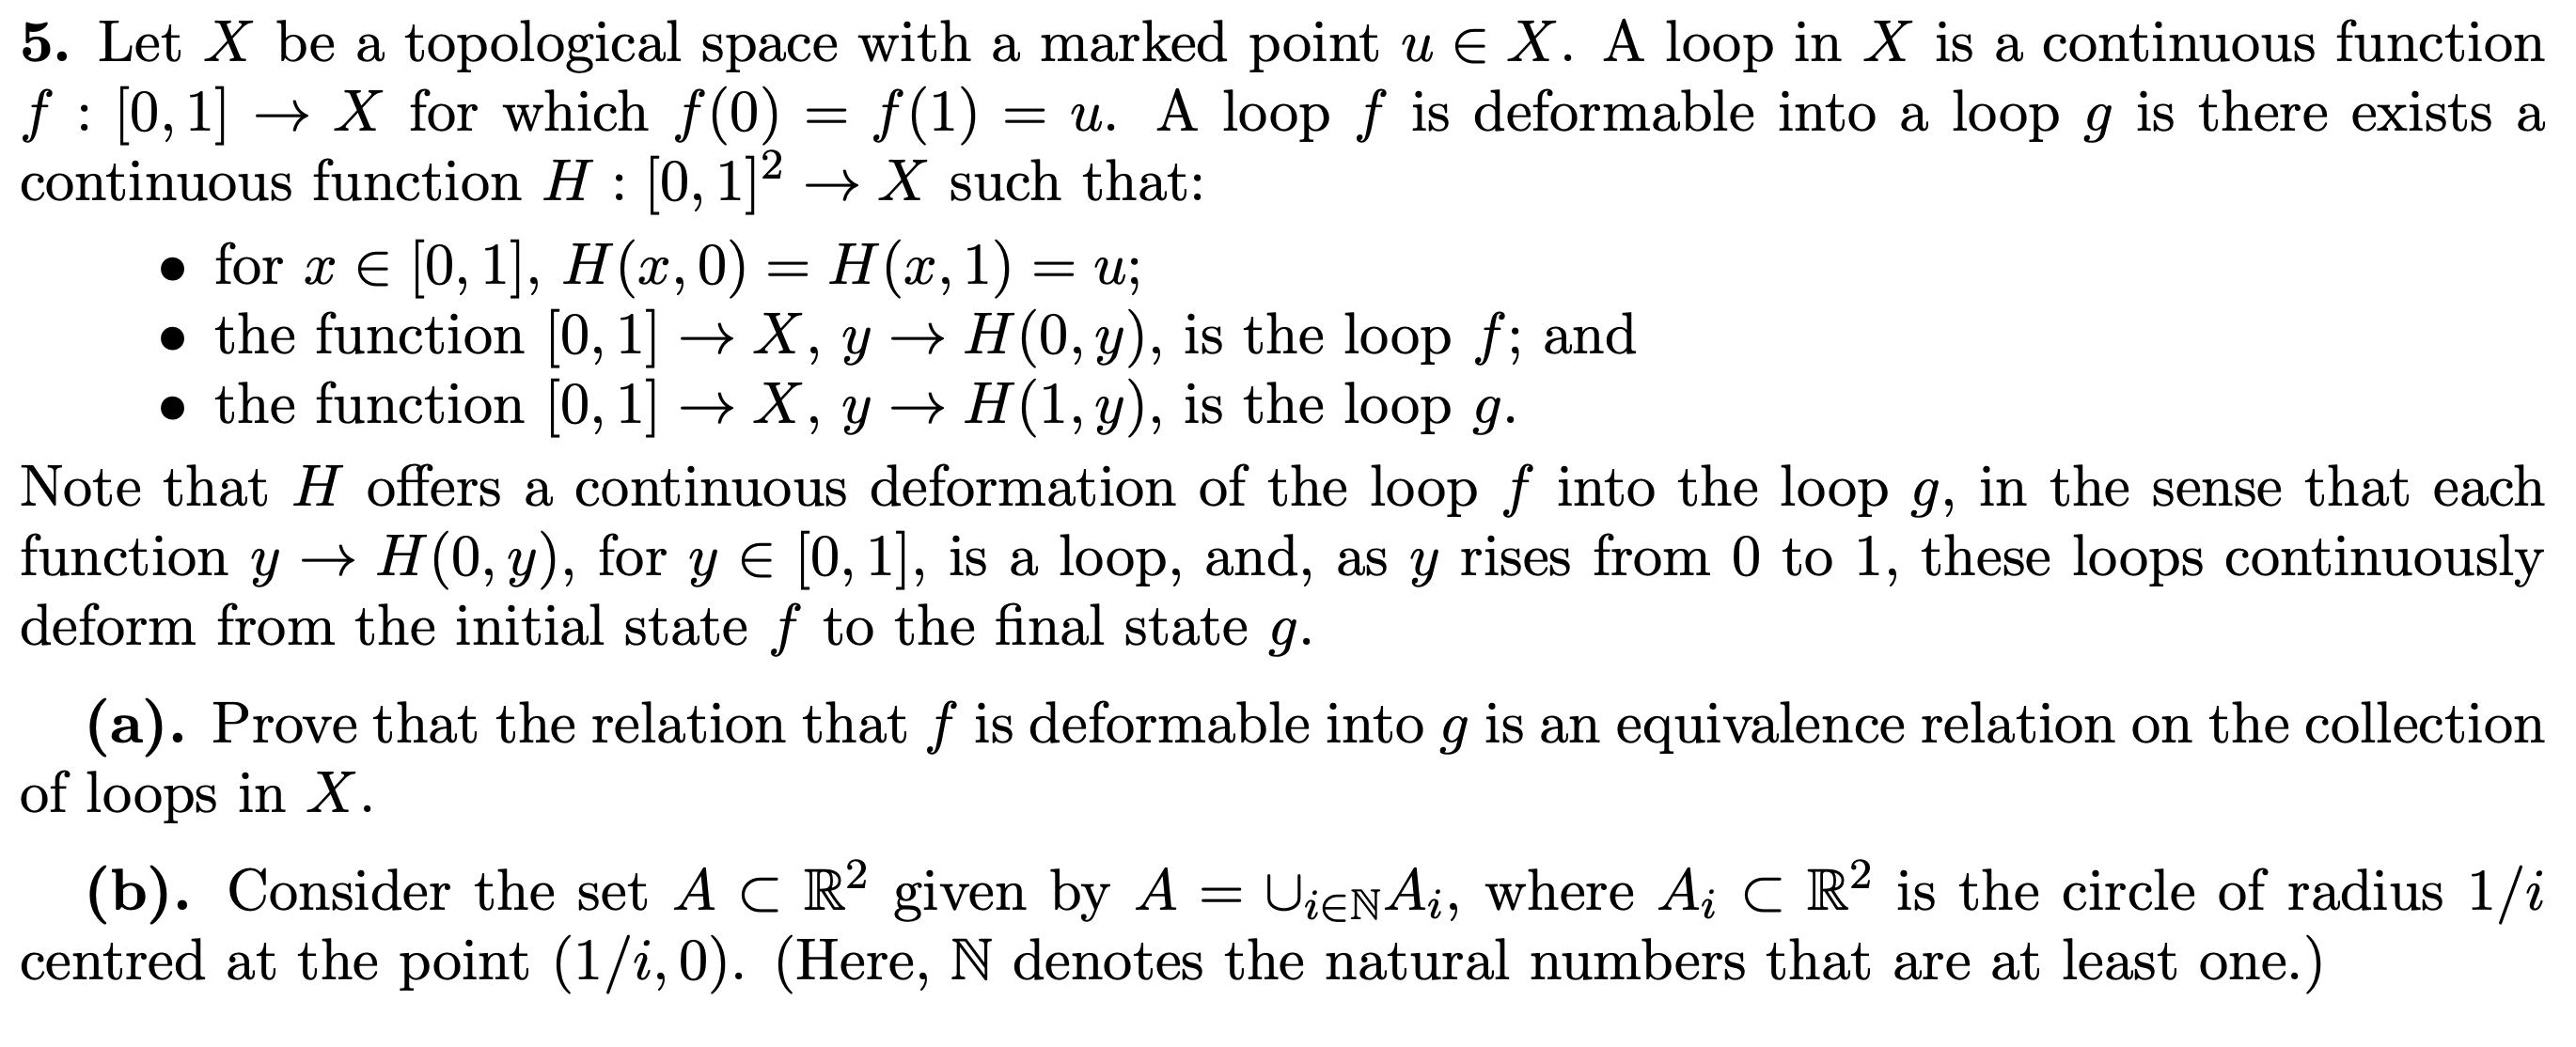
\includegraphics[width=400pt]{img/analysis--berkeley-202a-hw13-aa83.png}\\
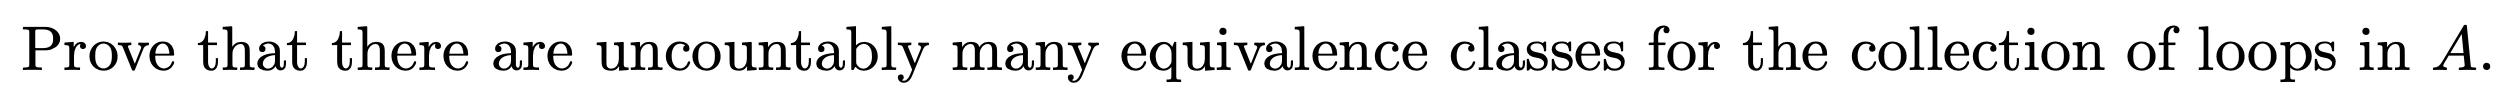
\includegraphics[width=400pt]{img/analysis--berkeley-202a-hw13-f49f.png}
\end{mdframed}

Note that $H$ offers a continuous deformation of the loop $f$ into the loop $g$, in the sense that each
function $y \to H(0, y)$, for $y$

Note that $H$ offers a continuous deformation of the loop $f$ into the loop $g$, in the sense that each
function $y \mapsto H(x, y)$, for $y \in [0, 1]$, is a loop. For $x = 0$ this is the loop $f$, and as $x$ rises
from $0$ to $1$, the loop continuously deforms from $f$ into $g$.

\begin{enumerate}[label=(\alph*)]

\item
  \begin{claim*}
    The relation $f$ is deformable into $g$ is an equivalence relation on the collection of loops in $X$.
  \end{claim*}

  \begin{proof}
    Let $\sim$ be the relation: $f$ is deformable into $g$.
    \begin{enumerate}

    \item {\it Reflexive}: yes, $f \sim f$ since we may take $H(x, y) = f(y)$ for all $x$.

    \item {\it Symmetric}: Let $H_{f,g}: [0, 1]^2 \to X$ be a function such that $f \sim g$.
      Then $H_{g,f} = \{((1 - x, y), H(x, y)) ~:~ x \in [0, 1], y \in [0, 1]\}$ is a function such
      that $g \sim f$.

    \item {\it Transitive}: Let $H_{f,g}: [0, 1]^2 \to X$ be such that $f \sim g$, and let
      $H_{g,h}: [0, 1]^2 \to X$ be such that $g \sim h$. Then
      \begin{align*}
        H_{f, h} =
        ~~~~&\Bigg\{ \(\(\frac{x}{2}, y\), H_{f, g}(x, y)\) ~:~ x \in [0, 1), y \in [0, 1]\Bigg\} \\
        ~~~~\union ~&\Bigg\{ \(\(\frac{1}{2} + \frac{x}{2}, y\), H_{g, h}(x, y)\) ~:~ x \in [0, 1], y \in [0, 1]\Bigg\}
      \end{align*}
      is a function such that $f \sim h$.
    \end{enumerate}
  \end{proof}

\item
  \begin{claim*}
    There are uncountably many equivalence classes for the collection of loops in $A$.
  \end{claim*}


  Informally: each loop corresponds to a countable sequence of circles each of which may be followed in one of
  two orientations (clockwise and anticlockwise). Loop $f$ is deformable into loop $g$ if their sequence of
  orientations are the same. This is in general a countably infinite binary sequence and hence there are
  uncountably many equivalence classes.

  \begin{proof}
    We define a loop in $A$ to be a continuous function $f: [0, 1] \to \R^2$ satisfying $f(0) = f(1) = (0, 0)$
    and $f([0, 1]) \subseteq A$.

    Let $\mc L = \{f_\gamma ~:~ \gamma \in \Gamma\}$ be the collection of loops in $A$.

    Let $K_\gamma = \big|\{t \in [0, 1) ~:~ f_\gamma(t) = (0, 0) \}\big|$ be the number of times
    loop $f_\gamma$ passes through $(0, 0)$ before $t = 1$, if this is finite. If the loop follows infinitely
    many circles then set $K_\gamma = \infty$. We have $K_\gamma \geq 1$ because each loop starts
    at $(0, 0)$.

    Note that a loop can follow infinitely many circles without needing to ``move at infinite
    speed'': for example, viewing $t \in [0, 1)$ as a time parameter, we may divide $t$ up
    as $\sum_{n=1}^\infty \frac{1}{2^n}$, i.e. specify that the particle spends a fraction $2^{-n}$
    of the total time traversing the $n$-th circle.

    Note that a circle may be followed in one of two ``orientations​'': clockwise or anticlockwise.
    Let $\rho_{\gamma, k}$ be the orientation of the $k$-th circle in loop $\gamma$.

    If $K_\gamma < \infty$ then set $\rho_{\gamma, k} = 0$ for all $k > K_\gamma$. Thus every loop $f_\gamma$
    is associated with an infinite sequence $\rho_1, \rho_2, \ldots$.

    Define the relation $f \sim g$ to mean $f$ is deformable into $g$. We have seen above that this is an
    equivalence relation.

    Let $\lambda, \gamma \in \Gamma$. We claim that $f_\gamma \sim f_\lambda$ if and only
    if $\rho_{\gamma, k} = \rho_{\lambda, k}$ for all $k \in \N$. In other words, two loops are equivalent if
    and only if the sequences of orientations of their circles are the same.

    \red{TODO}: make this topological argument.

    (Careful: there are finite loops (for which we have assigned an infinite tail of zeros), and also infinite
    loops which happen to have a tail of zeros.)

    Therefore the set of equivalence classes under $\sim$ is in bijection with the set of infinite binary
    sequences $\{(\rho_1, \rho_2, \ldots) ~:~ \rho_k \in \{0, 1\}\}$. Clearly, this is uncountable, since it is
    in bijection with the uncountable set $[0, 1] \subset \R$. Explicitly, let $\omega \in [0, 1]$ and
    let $d_1, d_2, \ldots$ be the binary expansion of the fractional part of $\omega$. If this expansion
    terminates after finitely many, say $J$, places, then set $d_j = 0$ for all $j > J$. Then we
    assign $\omega \mapsto (d_j)_{j=1}^\infty$. This is clearly injective, and also surjective since every
    possible binary expansion is realised by some $\omega \in [0, 1]$.
  \end{proof}
\end{enumerate}
